\externaldocument{1-introduction}

\chapter{Generic Offline Design}\label{chap:offline}
The implementation of distributed assertion checking on any blockchain requires some off-chain considerations and infrastructure. The previous chapter defined a formal set of logical formulae amenable for this approach and gave some in-depth examples. As was stated before, the proposed implementation in the following chapters is, for the most part, restricted to formulas of predicate logic using universal quantification.\\
The purpose of the offline infrastructure is to provide a syntax for stating assertions that check logical formulas, as well as a toolchain to compile these assertions into code that can be originated on the target blockchain. Depending on the individual solution for the respective blockchain, this can either be the original contract extended with the assertion code, or separate code that extends the contract in some other way. This chapter describes the generic part of the offline design, which corresponds to the front-end of the compilation pipeline shown in \figref{fig:pipeline_generic}. As a start, \secref{sec:syntax} describes the concrete syntax for writing assertions and shows how it expresses some of the previously given examples. The transformation of the original assertions to assertions that check for counterexamples is formalized in \secref{sec:transformation} \todo{how to handle proofs}. Lastly, \secref{sec:effectiveness} analyses the reliability of distributed assertion checking.

\section{Assertion syntax}
The assertion syntax is described in two versions by the EBNF grammars shown in appendix \ref{apx:grammar}. One version implements a prefix and the other one an infix notation. The pipeline currently supports the prefix notation with mandatory parentheses to avoid the need of handling operator precedences. To avoid context switches (at least for developers on Tezos), the assertion syntax references those of OCaml and Michelson.\\
A file containing assertions (henceforth called `assertion contract') contains at least one assertion for some function or entrypoint of the original contract (henceforth called `parent contract'). An assertion begins with a signature consisting of an optional tag followed by a parameter type declaration. The tag can be used for documentation, but may sometimes be needed to indicate to which function of the parent contract the assertion is assigned. The body is an (optional) nesting of quantifiers and conditions around exactly one assertion. Conditionals can be used to restrict the quantification domains or for some other constraints. For completeness, the existential quantifier is already included in the grammar, however the current version of the pipeline will reject any assertions containing it.\\
In order to make the front-end generic, the assertion grammar constitutes a union of operations and types for the target languages. This also allows the transformation to be oblivious of the target platform and be identical for all backends. The current version of the grammar recognizes all types present in the Tezos VM and a subset of operations that Michelson provides. Responsible for rejecting any assertions containing unsupported types or operations are the respective backends.

\subsection{Assertion example}
Consider a variation of the formula in predicate logic that checks whether a given list is sorted in ascending order:
\begin{equation}\label{eq:sorted_v2}
	(\forall n : int)(\forall m : int) (0 \leq n < m < |a|) \Rightarrow a[n] \leq a[m]
\end{equation}
A respective assertion that checks this property for the parent contract from \lstref{lst:sorted} could be expressed as follows:
\lstinputlisting[caption=Assertion checking if a list is sorted, language=Assertion, label={lst:sorted_assertion}]{listings/sorted.tza}

\subsection{Extensions}
In future iterations, the assertion syntax could be extended with some more features to improve usability and readability:
\begin{itemize}
\item \textbf{Local variables} to store, reuse and denominate computed values
\item \textbf{User-defined functions} to extract whole routines that can be reused in a single or even many assertion contracts, if defined as a module.
\item \textbf{if-else conditions} to modify the domains of quantification if certain conditions hold. The assertion that checks whether two numbers are relatively prime (discussed in \secref{sec:coprime}) is a good use-case for this feature in several ways. Firstly, the minimum of the given number has to be determined, however the \texttt{min}-function might not be supported as a built-in function by the target language (Tezos, for instance, does not support it). A solution for that could be to implement two branches in the program to handle each case. Secondly, if the greater of the two numbers is not evenly divided by the smaller one, the formula can be optimized by reducing the quantification domain by half to $(2 \le n \le \lfloor \frac{min(a,b)}{2} \rfloor)$, as a number cannot be evenly divided by any number between itself and its half \cite{bernhardt_veigel_2020}. With a syntax supporting a \texttt{if-else} control structure, the respective assertion could look as follows:
\lstinputlisting[caption=Assertion syntax with if-else structures \cite{bernhardt_veigel_2020}, language=Assertion, label={lst:coprime}]{listings/coprime_ifelse.tza}
This feature is not included in the current version, because conditional domain restrictions make the translation from quantifiers to random generators or loops more complex. Aside from that, without the feature of variables and user-defined functions, the code is inflated significantly, thus causing increased origination cost.
\end{itemize}

\section{Transformation}\label{sec:transformation}
Since the validators will check the input parameter for the negation of the formula, it has to be transformed before compilation. Furthermore, the formula should explicitly state the domain for each quantifier, which will have to be translated into a set of bounds that belong to the respective random generator. These restrictions are important in order to avoid wasting resources through testing values out of the relevant (or legal) scope.

\subsection{Negation}
The formula is negated using the negation rules of second-order logic and applying De Morgan's laws until the negation is applied to the literals. Negating universal quantification is equivalent to an existential quantification of its negated body (and vice versa): $\neg \forall x P(x) \equiv \exists x \neg P(x)$ \cite{Sundstrom2020Quantifiers}. The domain restrictions are not affected by the negation - the domain of the statement remains the same. This is also reflected in the rules of predicate logic, if the domain restrictions are given as a premise in the logical formula: $\neg (p \Rightarrow q) \equiv p \Rightarrow \neg q $.

\subsection{Defining the domain of random generators}
In order to assign each explicit bound to the respective quantifier, the formula has be skimmed for atomic constraints that contain bound variables. They're then moved and assigned to the quantifier that bounds the variable. If the constraint contains more than one, it is assigned to the quantifier with the highest depth in the order of quantifiers. \\
Consider a variation of the example given in \eqref{eq:sorted}, a formula checking if a given list is sorted:
\begin{equation}\label{eq:sorted_v2}
	(\forall n : int)(\forall m : int) (0 \leq n \le m < |a|) \Rightarrow a[n] \leq a[m]
\end{equation}
\todo{variation given above. refer to that}

The premise can be considered as a conjunction of the four constraints $0 \leq n$, $n < |a| $, $n \le m$ and $m < |a|$. Applying the rules given above after negating the formula, the constraints are assigned to the quantifiers as follows:
\begin{equation}\label{eq:sorted_v2_bounds}
	(\exists n : int, 0 \leq n \wedge n < |a|)(\exists m : int, m > n \wedge m < |a|) \text{ } a[n] > a[m]
\end{equation}
Ultimately, the quantifiers are then translated to the corresponding random generators shown in \lstref{lst:rand}.
\begin{lstlisting}[label=lst:rand]
n = random(0, size(list))
m = random(n, size(list))
\end{lstlisting}

While conjunctions can be handled easily, other operators make it more difficult to derive efficient random generators. Consider the following constraints:
\begin{align}
(\forall n : int) (n < 10 \lor n > 20) ... \\
(\forall n : int) (n \ne 10) ... \\
(\forall n : int) (n = 10) ... 
\end{align}

Both constraints 1) and 2) complicate restricting the random generator in several ways. Firstly, they separate the domain into two disjoint sub-domains, which requires defining a random generator for each range and another one to decide which one is called. Secondly, the operands of a disjunction cannot be considered separately when more than one bound variable is involved. For the predicate whose random generator is executed first, the domain restriction is optional, while the generation of the following random values depend on the previous result. As the complexity of building efficient random generators in these cases is relatively high, restrictions formulated with these operators are kept, for now, as part of the assertion code rather than used as constraints for the generators. Consequently, some validators may generate irrelevant values when checking the assertion. Depending on the size of the gap between the sub-domains, this can significantly decrease the reliability of this kind of assertion checking. Constraint 3) effectively makes the quantifier, which binds $n$, obsolete. Adding this constraint to the respective generator will at least not affect the reliability, but a future improvement could be to optimize the assertion by replacing all occurrences of the bound variable with the assigned value and removing the quantification.\\

In some cases, boundaries are given implicitly by data types. List indices, for instance, are always bound to the range $0.. size(list) - 1$ and could thus be derived from the formula without an explicit specification. As this deduction makes the transformation more complex, as it requires a semantic analysis of the formula, a completely explicit formula in terms of the domain is required for now. Depending on the virtual machine, the lower bound for indexing operations can be handled by the random generator of an appropriate predicate type. As an example, Michelson supports the data type \texttt{nat} representing the natural numbers, which categorically excludes all values below zero. Developers aware of this can exploit this and, for instance, abbreviate \eqref{eq:sorted_v2} with the following formula:
\begin{equation}\label{eq:sorted_v2_abbr}
	(\forall n : nat)(\forall m : nat) (n \le m < |a|) \Rightarrow a[n] \leq a[m]
\end{equation}

\section{Accuracy of the approach}
Since the proposed approach implements a probabilistic test, its accuracy as well as the costs incurred by guaranteeing a specified certainty threshold, remains to be analysed. The goal is to identify a formula that, given the domain of a formula in predicate logic, returns an estimate of a lower bound of samples necessary to find an existing counterexample with a probability $p$. From this analysis, it can be derived how effective a formula can be checked on a blockchain with $m$ validators. For the remainder of this chapter, the assumptions hold that the random generator picks elements independently from a uniform distribution and that there exists exactly one counterexample for the passed parameter.\\
The following two sections depict the findings from \cite{bernhardt_veigel_2020}.
\todo{further measures for blockchains with small number of validators}
\todo{Refer to our example paper}

\subsection{Coupon Collector Problem Analysis}
When checking properties with probabilistic testing, the result is either definitely not satisfied, or probably satisfied. Thus, errors only occur as false positives. In order to find an existing counterexample with $p = 1$, every element in the given domain $\mathcal{D}$ has to be checked by at least one validator. Deterministically, this is reachable with exactly $|\mathcal{D}|$ test runs. This is, however, invalid for the probabilistic approach, as some validators may generate duplicate random values and leave some elements of $\mathcal{D}$ unchecked. \\
In probability theory, this is known as the Coupon Collector's Problem \cite{croucher_collecting_2006}. Given $n = |\mathcal{D}|$, the probability that no duplicate elements are generated is given by
\begin{equation*}
    p = \prod_{i=1}^{n} \frac{i}{n}
\end{equation*}
As an example, the probability that all validators generate a unique random value already drops to $0.036\%$ for $n = 10$. Let the random variable $T$ be number of test runs executed until every element in the domain has been checked. The goal is to identify its expectation $E(T)$. To this end, the geometric probability distribution is applied \cite{croucher_collecting_2006}:\\
Each element is generated with a probability of $1/n$. Thus, the probability to generate the $i$th unique element is given by 
\begin{equation}
    p_i = \frac{n-i+1}{n}
\end{equation}
The expected value of a random variable $X$ is given by $E(X) = \frac{1}{p}$\cite{croucher_collecting_2006}, thus the expected number of test runs for $n$ is 
\begin{equation}
E(T) = n \sum_{i=1}^{n} \frac{1}{i}
\end{equation}
\tabref{tab:prob_outcomes} shows the expected number of test runs $E(T)$ and its standard deviation $\sigma$ for different $n$. In \cite{croucher_collecting_2006}, $E(T)$ and $\sigma$ and the application of the central limit theorem are used to calculate a 95\% confidence interval for $T$, which provides an upper and lower bound on the number of test runs. Rounded values for both bounds are also shown in \tabref{tab:prob_outcomes}.
\begin{table}[h]
    \centering
    \begin{tabular}{lllll}\label{tab:prob_outcomes}
        \thead{$n$} & \thead{$E(T)$} & \thead{$\sigma$} & \thead{lower bound} & \thead{upper bound}\\ \hline
        5 & 11.4 & 2.53 & 6 & 16\\
        10 & 29.3 & 4.32 & 21 & 38\\
        20 & 72.0 & 7.21 & 58 & 86\\
        30 & 119.8 & 9.48 & 101 & 138 \\
        50 & 225.0 & 13.23 & 199 & 251 
    \end{tabular}
    \caption{Expectation, standard deviation and upper and lower bound of needed test runs for some $n$ \cite{croucher_collecting_2006}}
    \label{tab:my_label}
\end{table}

The results show that checking random values is a very inefficient approach if false positives are not admissible. Even if the lower bound of $T$ is chosen as the number of test runs, it exceeds the size of the domain by far and increases the time complexity to $\mathcal{O}(n*log(n))$ for large $n$ \cite{xu_tang_2011}. Instead, the following section introduces a formula to calculate the number of test runs that detect counterexamples with a $p < 1$, for instances where false positives are tolerable.

\subsection{Setting probability thresholds}
The goal is to find a number $t$ of test runs, s.t. the probability $P_{c,t}$ of not finding the counterexample drops below a certain threshold $c$. A validator finds the counterexample in one test run with probability $\frac{1}{n}$, and misses it with probability $(1-\frac{1}{n})$. After $t$ tests runs, the probability that the counterexample has not been found is thus $(1-\frac{1}{n})^t$. Following the same approach as in \cite{mahl_schindel_2007} to retrieve a bound for $P_{c,t}$, we use
\begin{equation}
(1-\frac{1}{m})^m \leq \frac{1}{e}
\end{equation}
which holds for all $m > 0$. From this inequality, it follows that
\begin{equation}
(1-\frac{1}{n})^t = ((1-\frac{1}{n})^n)^{\frac{t}{n}} \le e^{-\frac{t}{n}}
\end{equation}
With this, the probability $P_{c,t}$ of not finding the counterexample with $t$ test runs can be defined as
\begin{equation}
P_{c,t} \le e^{-\frac{t}{n}}
\end{equation}
In order to retrieve the number of test runs $t$ necessary for $P_{c,t}$ to drop below a specified threshold $c$, the inequality is solved for $t$, which depends on the known parameter $n$ and an arbitrary value for $c$:
\begin{align}
    e^{-\frac{t}{n}} &\leq c && \text{with } c\le1 \nonumber\\
    t &\geq -n\:\ln(c)
\end{align}
For $c = \frac{1}{e}$ ($\approx 36.79\:\%$) $t$ is bound by $n$, which means that for higher reliabilities the number of test runs needs to be greater than $n$. \figref{fig:graph_t_c} shows the lower bounds of $t$ as a function of the probability threshold and domain size. One can see that the increase in accuracy is approximately linear to the number of test runs below a threshold of $c=0.5$, but requires an exponential testing effort to reach higher thresholds.
\begin{figure}[h]
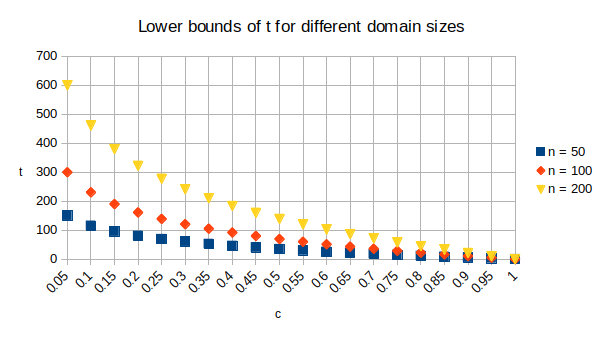
\includegraphics[width=0.95\linewidth]{figures/3-offline/graph_t_c}
\label{fig:graph_t_c}
\end{figure}
For assertions with several quantifiers, which are translated to random generators, all domains have to be considered in the calculation. Revisiting the intersection of sets from \secref{sec:existential}, every element in set $u$ has to be compared to every element in set $v$. Thus, the lower bound of test runs needed to check they intersect with a certainty of 63.21\% is given by $t \leq t_1 * t_2$ with $t_1 \leq |u|$ and $t_2 \leq |v|$.

\subsection{Validators vs. test runs}
The last section derived a formula to calculate a lower bound for a number of test runs $t$ in order to reach a certain level of confidence. However, $t$ is not a parameter that can be adjusted to an arbitrary value on the blockchain, as the assertion is checked by the validators. Assuming a blockchain has $m$ validators, the actual lower bound of test runs is $m$. For cases where there are not enough validators to reach a threshold $c$, a mechanism is required to have each validator to check the property for multiple random values. Hence, the actually executed number of checks is always a multiple of $m$. 

\subsection{Alternatives to random testing}
For applications where higher reliability is crucial, an alternative to checking elements randomly could be to coordinate a systematic iteration of the domain. The implementation of such a coordination is not trivial though; validators can't simply be passed an individual value as input. Instead, possible approaches could be to implement a central instance that allocates an element in the search space to each validator, or use some unique and intrinsic attribute, like an identification number, as input for a mapping.

\subsubsection{Central instance assigning values}
For this approach, the tool-chain would need to generate a separate contract that is called by the baker and validators as a proxy. This contract would then, for instance, generate a number using a modulo-n counter and pass this number as an additional parameter to the assertion code. The random generators would be omitted accordingly. However, this works only as expected if there are no simultaneous transactions calling the contract, otherwise it cannot be guaranteed that all elements have been assigned for each transaction. If and how this issue can be solved will not be discussed further in this thesis.

\subsubsection{Using unique attributes of a validator}\label{sec:alt_attributes}
This approach strongly depends on whether the validators have a unique id or other attribute that can be accessed from within a contract.  If there is (or the language can be extended with such a feature), there needs to exist a non-injective surjective function that maps the respective attributes represented by type A to an element of the domain represented by type B. Furthermore, for cases where $t > m$, an offset needs to be added, s.t. a validator checks distinct elements for each test run. \\
Implementing such an approach on Tezos does become even more challenging by the way endorsing rights are distributed in its proof-of-stake mechanism: for each block level, endorsing rights are assigned to the owner of a randomly selected roll, i.e., a set of tokens \cite{tezos_docs}. This means that the same endorser can be picked multiple times for endorsing one block and thus some elements in the domain may remain unchecked. \secref{lala} goes into more detail about this issue. \todo{Ref section}